\section{Discussion of results}%
\label{sec:result_discussion}

\todo[inline]{What are the limiting factors? Data statistics /
  statistical precision of the bkg estimate (could be improved with a
  better data-driven background estimate).}

\todo[inline]{Systematic uncertainty relatively unimportant at this
  stage.}

\subsection{Search for non-resonant production of Higgs boson pairs}


\begin{figure}[htbp]
  \centering

  \begin{subfigure}{0.53\textwidth}
    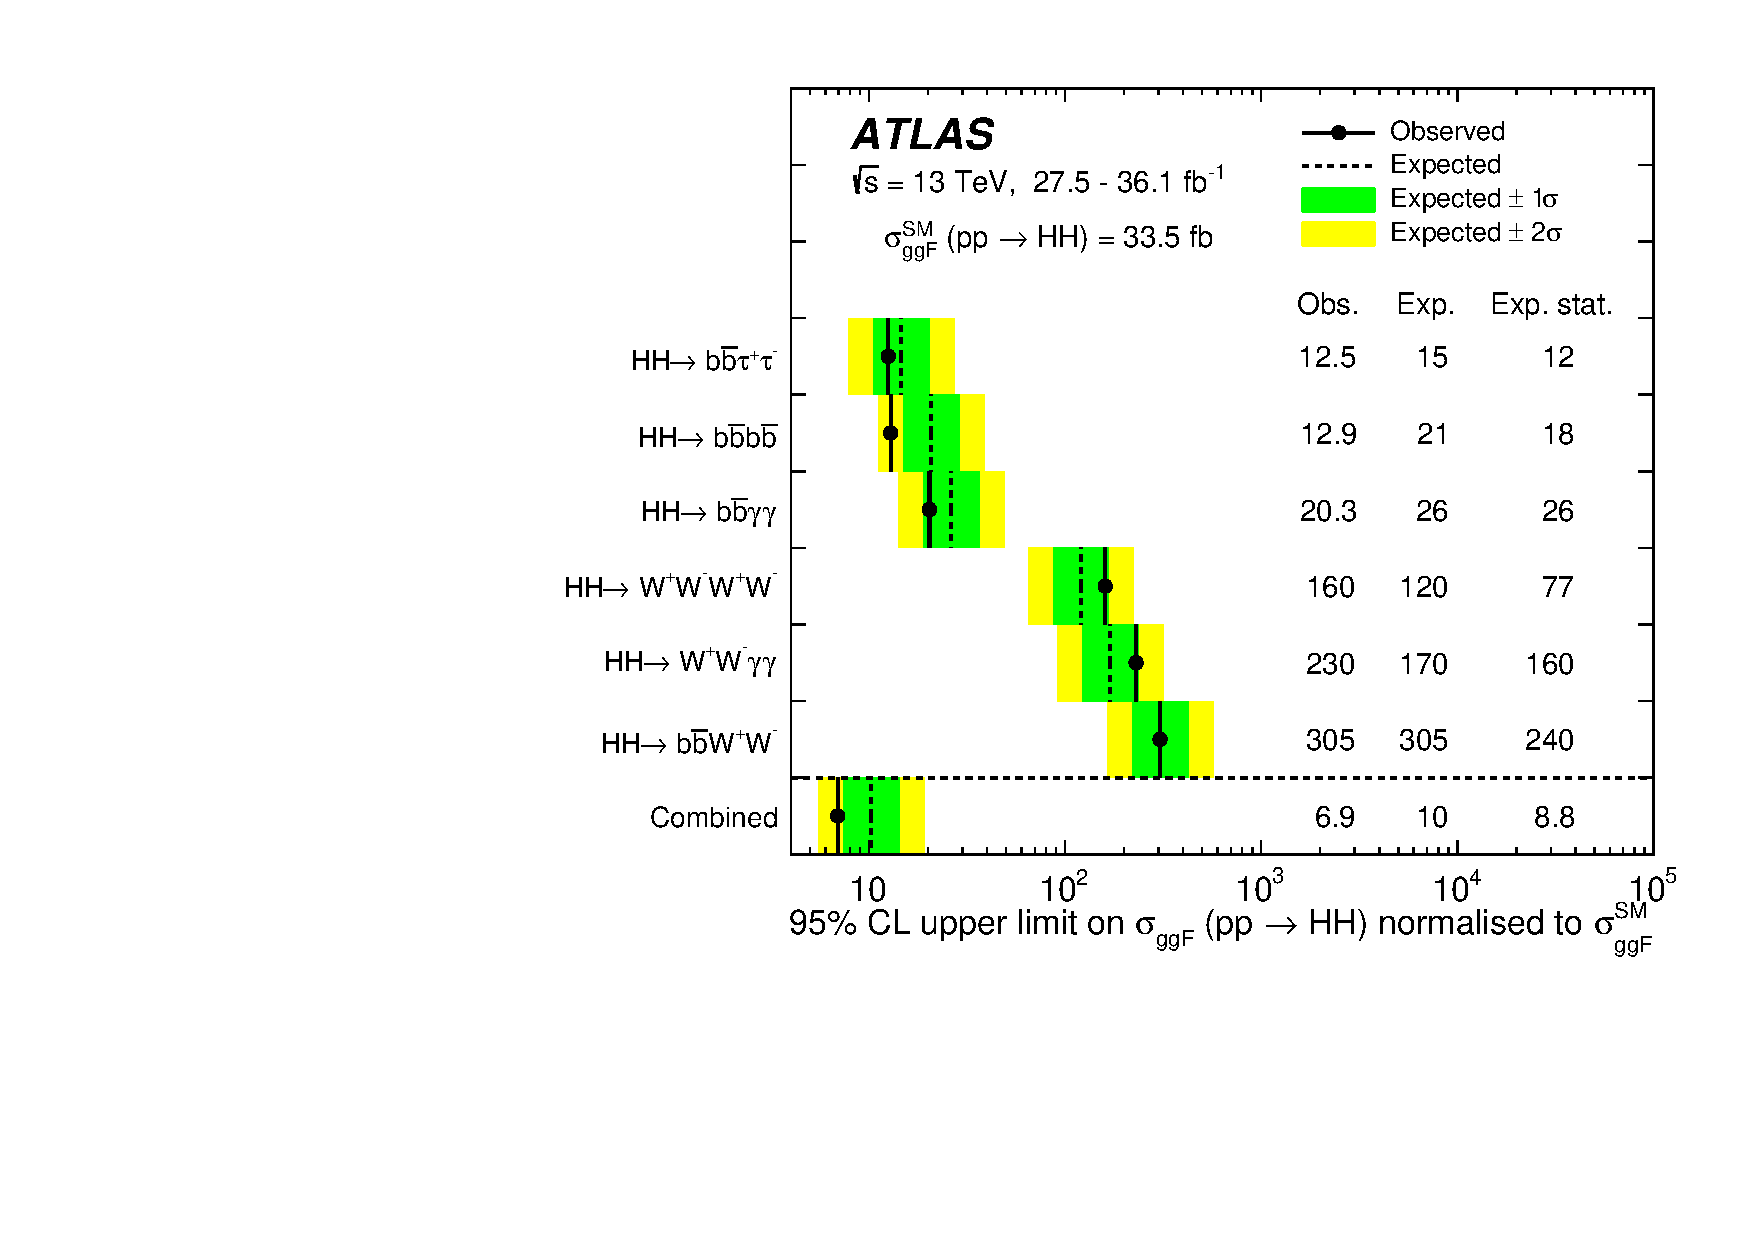
\includegraphics[width=\textwidth]{discussion/results_36ifb}
    \subcaption{Partial Run~2 dataset with an integrated luminosity of \num{27.5} -
      \SI{36.1}{\per\femto\barn}~\cite{HDBS-2018-58}}
  \end{subfigure}\hfill%
  \begin{subfigure}{0.45\textwidth}
    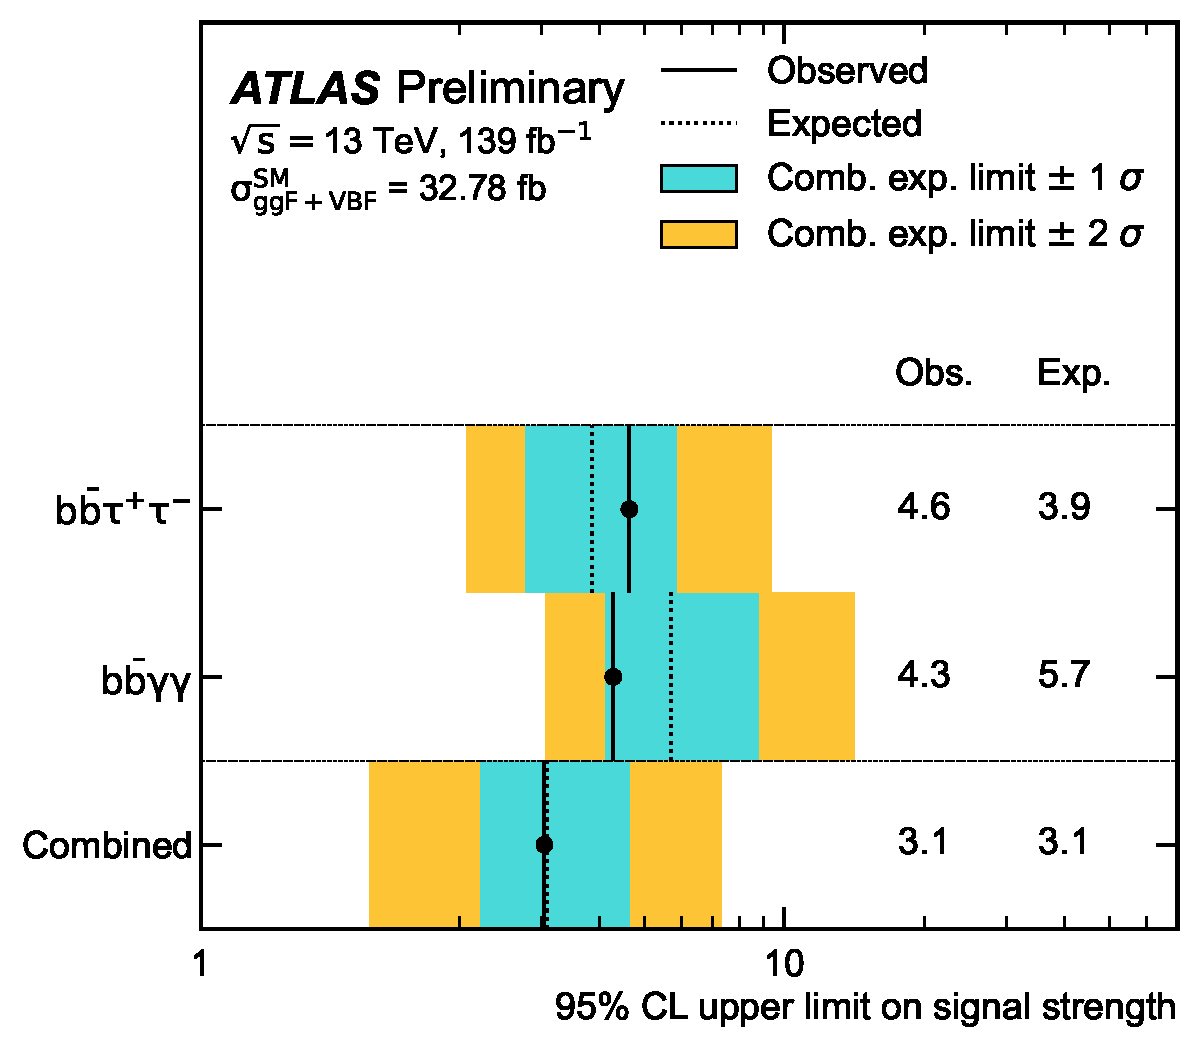
\includegraphics[width=\textwidth]{discussion/results_139ifb}
    \subcaption[margin=5em]{Full Run~2 dataset with an integrated luminosity
      of~\SI{139}{\per\femto\barn}~\cite{ATLAS-CONF-2021-052}}
  \end{subfigure}

  \caption{Comparison of
    Results
    Non-resonant results. Note different POIs and cross
    sections. Note the different results for bbtautau.}
  \label{fig:blabla}
\end{figure}


\begin{table}[htbp]
  \centering

  \begin{tabular}{l@{\hskip 2em}SSc}
  \toprule
  \textbf{CMS} (\SI{138}{\per\femto\barn}) & \multicolumn{3}{c}{Upper limit on $\mu_{gg\text{F+VBF}}$ (\SI{95}{\percent} CL)} \\
  \cmidrule{2-4}
  Final state & {Observed} & {Expected} & Reference \\
  \midrule
  $\bbbar\tau^{+}\tau^{-}$ & 3.3 & 5.2 & \cite{CMS-PAS-HIG-20-010} \\
  $\bbbar\gamma\gamma$ & 7.7 & 5.2 & \cite{CMS-HIG-19-018} \\
  $\bbbar\bbbar$ & 3.9 & 7.8 & \cite{CMS-HIG-20-005-PREPRINT} \\
  % Multilepton = ($W^+W^-W^+W^-$, $W^+W^-\tau^+\tau-$, $\tau^+\tau^-\tau^+\tau^-$)
  Multi-lepton  & 21.8 & 19.6 & \cite{CMS-PAS-HIG-21-002} \\
  \bottomrule
\end{tabular}


%%% Local Variables:
%%% mode: latex
%%% TeX-master: "../phd_thesis"
%%% End:


  \caption{CMS results for non-resonant HH search}
  \label{tab:cms_nonresonant}
\end{table}


\begin{itemize}
\item Why is hadhad more sensitive?
\item How do these results compare to other channels / CMS at the end of Run 2?
\end{itemize}

Improvements with respect to the previous analysis. Outscaling lumi...

How does the excess fit into other results?

$4b$: \SI{6.5}{\femto\barn} (exp.\ \SIpmerr{8.15}{+1.17}{-0.77}{\femto\barn})

\todo[inline]{Discussion excess: Modelling of collinear taus?}





\subsection{Search for resonant production of Higgs boson pairs}

%%% Local Variables:
%%% mode: latex
%%% TeX-master: "../../phd_thesis"
%%% End:
